% Native vector artwork; positions are in centimetres.
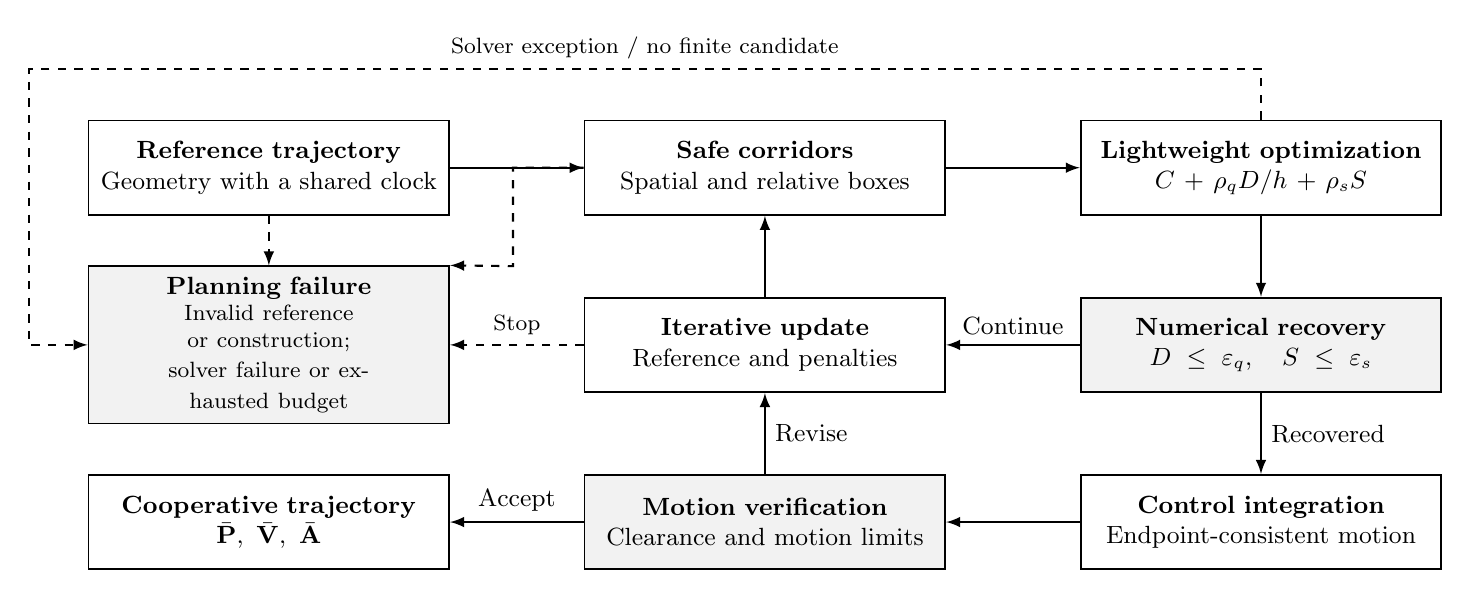
\begin{tikzpicture}[x=1cm,y=1cm,>=latex,font=\small,
 block/.style={draw=black,line width=.65pt,fill=white,text width=4.3cm,minimum height=1.2cm,inner sep=4pt,align=center},
 test/.style={draw=black,line width=.65pt,fill=black!5,text width=4.3cm,minimum height=1.2cm,inner sep=4pt,align=center},
 flow/.style={->,line width=.75pt}]
\node[block] (ref) at (0,0) {\textbf{Reference trajectory}\\Geometry with a shared clock};
\node[block] (corr) at (6.3,0) {\textbf{Safe corridors}\\Spatial and relative boxes};
\node[block] (qp) at (12.6,0) {\textbf{Lightweight optimization}\\$C+\rho_q D/h+\rho_s S$};
\node[block] (update) at (6.3,-2.25) {\textbf{Iterative update}\\Reference and penalties};
\node[test,minimum height=1.35cm] (fail) at (0,-2.25) {\textbf{Planning failure}\\\footnotesize Invalid reference or construction;\\solver failure or exhausted budget};
\node[test] (gate) at (12.6,-2.25) {\textbf{Numerical recovery}\\$D\leq\varepsilon_q,\quad S\leq\varepsilon_s$};
\node[block] (control) at (12.6,-4.5) {\textbf{Control integration}\\Endpoint-consistent motion};
\node[test] (check) at (6.3,-4.5) {\textbf{Motion verification}\\Clearance and motion limits};
\node[block] (out) at (0,-4.5) {\textbf{Cooperative trajectory}\\$\bar{\mathbf P},\ \bar{\mathbf V},\ \bar{\mathbf A}$};
\draw[flow] (ref)--(corr);
\draw[flow] (corr)--(qp);
\draw[flow] (qp)--(gate);
\draw[flow] (gate.west)--node[above]{Continue}(update.east);
\draw[flow] (update.north)--(corr.south);
\draw[flow] (gate.south)--node[right]{Recovered}(control.north);
\draw[flow] (control.west)--(check.east);
\draw[flow] (check.north)--node[right]{Revise}(update.south);
\draw[flow] (check.west)--node[above]{Accept}(out.east);
\draw[flow,dashed] (ref.south)--(fail.north);
\draw[flow,dashed] (update.west)--node[above,font=\footnotesize]{Stop}(fail.east);
\draw[flow,dashed] (corr.west)--(3.1,0)--(3.1,-1.25)--(fail.north east);
\draw[flow,dashed] (qp.north)--(12.6,1.25)
 --node[above,font=\footnotesize]{Solver exception / no finite candidate}(-3.05,1.25)
 --(-3.05,-2.25)--(fail.west);
\end{tikzpicture}
